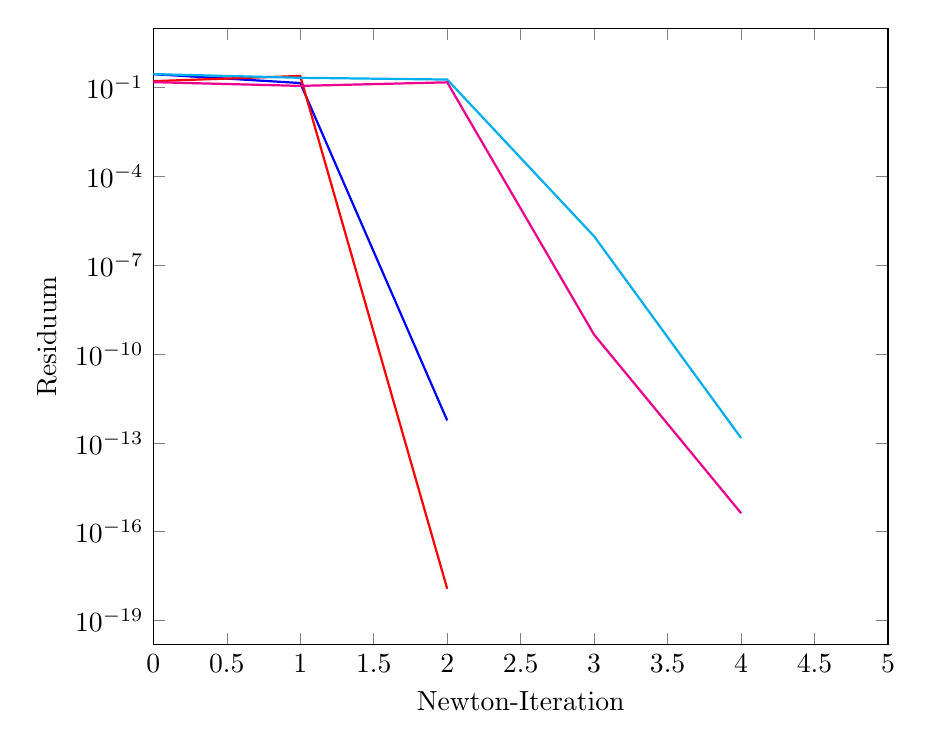
\begin{tikzpicture}[every plot/.append style={thick}] 
\begin{axis}[ 
label style={font=\normalsize}, 
xlabel={Newton-Iteration}, 
ylabel={Residuum}, 
xmin=0, xmax=5, 
ymode=log, 
ymin=0, ymax=10, 
width=0.9\textwidth, 
grid style=dashed, 
] 
\addplot[ 
color=blue, 
] 
coordinates { 
(0, 2.81e-01)(1, 1.41e-01)(2, 5.72e-13)}; 
\addplot[ 
color=red, 
] 
coordinates { 
(0, 1.63e-01)(1, 2.45e-01)(2, 1.18e-18)}; 
\addplot[ 
color=cyan, 
] 
coordinates { 
(0, 2.82e-01)(1, 2.12e-01)(2, 1.85e-01)(3, 9.37e-07)(4, 1.45e-13)}; 
\addplot[ 
color=magenta, 
] 
coordinates { 
(0, 1.51e-01)(1, 1.13e-01)(2, 1.49e-01)(3, 4.47e-10)(4, 4.21e-16)}; 
\end{axis} 
\end{tikzpicture} 
